\section{Hybrid Schedules} \label{sec:schedule}

This section describes how \peregrine computes (\S\ref{sec:compute-schedule})
and enforces (\S\ref{sec:enforce-schedule}) hybrid schedules.

\subsection{Computing Hybrid Schedules} \label{sec:compute-schedule}

To compute a hybrid schedule, \peregrine first extracts a total order of
synchronization operations from an execution trace.  Currently, it
%\peregrine
considers 28 \v{pthread} operations, such as \v{pthread\_mutex\_lock()}
and \v{pthread\_cond\_wait()}.  It also considers
the entry and exit of a thread as synchronization operations so that it can
order these events together with other synchronization operations.  These
operations are sufficient to run the programs evaluated, and more can be
easily added.  \peregrine uses a total, instead of a partial, order because
previous work has shown that a total order is already
efficient~\cite{cui:tern:osdi10,kendo:asplos09}.

\begin{figure}[t]
\centering
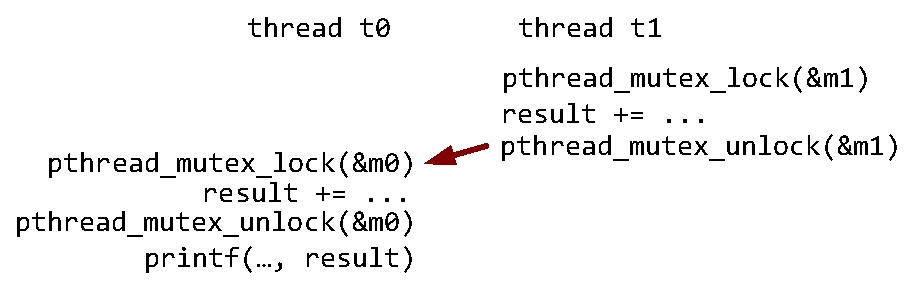
\includegraphics[width=.9\columnwidth]{peregrine/figures/concurrent-intervals.eps}
\caption{{\em No \peregrine race with respect to this
    schedule.}} \label{fig:concurrent-intervals}
\end{figure}

For determinism, \peregrine must detect races that occurred during the recorded
execution and compute execution order constraints to deterministically
resolve the races.  An off-the-shelf race detector would flag too many
races because it considers the original synchronization
constraints of the program, whereas \peregrine wants to detect races according
to a sync-schedule~\cite{pres:sosp09,recplay:tocs}.  To illustrate,
consider Figure~\ref{fig:concurrent-intervals}, a modified sync-schedule
based on the one in Figure~\ref{fig:trace}.  Suppose the two threads
acquire different mutex variables, and thread $t_1$ acquires and releases
its mutex before $t_0$.  Typical lockset-based~\cite{savage:eraser}
or happens-before-based~\cite{lamportclock} race detectors would flag a
race on \v{result}, but our race detector does not: the sync-schedule
in the figure deterministically resolves the order of accesses to \v{result}.  
Sync-schedules anecdotally reduced the number of
possible races greatly, in one extreme case, from more than a million to
four~\cite{pres:sosp09}.


%% For instance, consider the sync-schedule in
%% Figure~\ref{fig:concurrent-intervals}.  We use $T_{m,n}$ to denote the
%% region of an execution trace executed by thread $T_m$ between this
%% thread's $(n-1)^{th}$ and $n^{th}$ synchronization operation.  By
%% enforcing the sync-schedule between unrelated operations on lock \v{l1}
%% and \v{l2}, we effectively make region $T_{1,1}$ happens-before $T_{2,2}$
%% and $T_{2,1}$ happens-before $T_{1,3}$.  Thus, we do not need to detect
%% races for these regions.  Such sync-schedules can vastly reduce the number
%% of possible races, in one extreme case, from more than a million to
%% four~\cite{pres:sosp09}.

%% \peregrine constructs a happens-before graph,
%% such as the graph in Figure~\ref{fig:concurrent-intervals}, by adding a
%% directed edge for each pair of adjacent synchronization operations in a
%% sync-schedule.  It then iterates through each pair of concurrent regions
%% defined by the happens-before graph, and flags two instructions from these
%% regions respectively as a race if they access the same memory location and
%% at least one is write.

Mechanically, \peregrine detects occurred races using a happens-before-based
algorithm.  It flags two memory accesses as a race iff (1) they access the
same memory location and at least one is a \v{store} and (2) they are
\emph{concurrent}.  To determine whether two accesses are concurrent,
typical happens-before-based detectors use vector
clocks~\cite{vectorclock} to track logically when the accesses occur.
Since \peregrine already enforces a total synchronization order, it uses a
simpler and more memory-efficient logical clock representation.

Specifically, given two adjacent synchronization operations within one
thread with relative positions $m$ and $n$ in the sync-schedule, \peregrine uses $[m,n)$ as
  the logical clock of all instructions executed by the thread between the
  two synchronization operations.  For instance, in
  Figure~\ref{fig:trace}, all instructions run by thread $t_0$
  between the \v{pthread\_mutex\_unlock()} operation and the thread exit have
  clock $[4, 8)$.
%  where $4$ and $8$ are the relative positions of the    \v{pthread\_mutex\_unlock()} operation and the thread exit in the sync-schedule.
    \peregrine considers two accesses with clocks $[m_0, n_0)$
      and $[m_1, n_1)$ concurrent if the two clock ranges overlap, \ie,
        $m_0 < n_1 \wedge m_1 < n_0$.  For instance, $[4, 8)$ and $[5,
            6)$ are concurrent.

To deterministically resolve a race, \peregrine enforces an execution order
constraint $inst_1 \rightarrow inst_2$ where $inst_1$ and $inst_2$ are the
two dynamic instruction instances involved in the race.  \peregrine identifies a
dynamic instruction instance by $\langle sid, tid, nbr \rangle$ where
$sid$ refers to the unique ID of a static instruction in the executable
file; $tid$ refers to the internal thread ID maintained by \peregrine, which
always starts from zero and increments deterministically upon each
\v{pthread\_create()}; and $nbr$ refers to the number of control-transfer
instructions (branch, call, and return) locally executed within the thread
from the last synchronization to instruction $inst_i$.  For instance, \peregrine
represents the execution order constraint in
Figure~\ref{fig:trace} as $\langle L15,t_1,0\rangle \rightarrow
\langle L9,t_0,2 \rangle$, where the branch count $2$ includes the return
from \v{worker} and the branch L7 of thread $t_0$.
We must distinguish different dynamic instances of a static instruction
because some of these dynamic instances may be involved in races while others
are not.  We do so by counting branches because if an instruction is
executed twice, there must be a control-transfer between
the two instances~\cite{smp-revirt:vee08}.  We count branches starting from the last
synchronization operation because the partial schedule preceding this
operation is already made deterministic.


%% These branch instructions include LLVM instructions \v{br} (direct conditional
%% or unconditional branch), \v{switch}, \v{indirectbr}, \v{call}, and
%% \v{invoke} (like call instruction, but with a callee that may throw
%% exceptions).  

\begin{figure}[t]
\centering
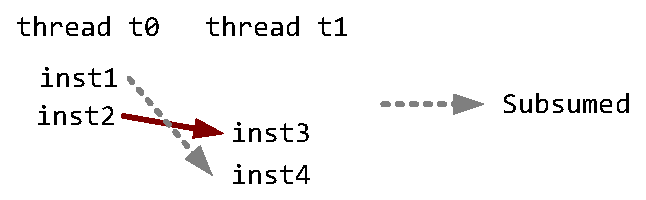
\includegraphics[width=.65\columnwidth]{peregrine/figures/pruned-order}
\caption{{\em Example subsumed execution order
    constraint.}} \label{fig:subsumed}
\end{figure}

If one execution order constraint subsumes another, \peregrine does not add the
subsumed one to the schedule.  Figure~\ref{fig:subsumed} shows a subsumed
constraint example.  Algorithmically, \peregrine considers an execution order
constraint $inst_1 \rightarrow inst_4$ subsumed by $inst_2 \rightarrow
inst_3$ if (1) $inst_1$ and $inst_2$ have the same logical clock (so they
must be executed by the same thread) and $inst_2$ occurs no earlier than
$inst_1$ in the recorded execution trace; (2) $inst_3$ and $inst_4$ have
the same logical clock and $inst_3$ occurs no later than $inst_4$ in the
trace.  This algorithm ignores
%considers only direct order constraints and 
transitive order constraints, so it may miss some subsumed constraints.
For instance, it does not consider $inst_1 \rightarrow inst_4$ subsumed if
we replace constraint $inst_2 \rightarrow inst_3$ with $inst_2 \rightarrow
inst_{other}$ and $inst_{other} \rightarrow inst_3$ where $inst_{other}$
is executed by a third thread.
% and keep other things unchanged.

\subsection{Enforcing Hybrid Schedules} \label{sec:enforce-schedule}

To enforce a synchronization order, \peregrine uses a technique called
\emph{semaphore relay}~\cite{cui:tern:osdi10} that orders synchronization
operations with per-thread semaphores.
At runtime, a synchronization wrapper
(recall that \peregrine instruments synchronization operations for runtime
control) waits on the semaphore of the current thread.  Once it is woken
up, it proceeds with the actual synchronization operation, then wakes up
the next thread according to the synchronization order.  
% Compared to an approach using locks or condition variables, semaphore
% relay avoids unnecessary lock contentions.
For programs that frequently do synchronization operations, the overhead
of semaphore may be large because it may cause a thread to block.  Thus,
\peregrine also provides a spin-wait version of
semaphore relay called \emph{flag relay}.
%% Specifically, a synchronization wrapper spin-waits on a
%% cache-aligned integer flag dedicated for the current thread, and sets the
%% flag for the next thread when its done.  Flag relay 
This technique turns out to be very
fast for many programs evaluated (\S\ref{sec:efficient}).

%% For an execution order constraint, \peregrine uses a more involved method
%% because one static instruction may have many dynamic instances.  Recall
%% that an execution order constraint has the form $inst_1 \rightarrow
%% inst_2$ where $inst_i$ are the two dynamic instruction instances
%% identified by thread ID, branch count, and static instruction ID
%% (\S\ref{sec:schedule}).  Thread ID is a deterministic thread ID maintained
%% by \peregrine.  Branch count counts locally within the thread the number of
%% branch instructions from the last synchronization operation to $inst_i$.  

% if we have space, include the slot function.

To enforce an execution order constraint, \peregrine uses program
instrumentation, avoiding the need for special hardware, such as the often
imprecise hardware branch counters~\cite{smp-revirt:vee08}.
% a more involved method to ensure that the order constraint is enforced
% on the right dynamic instance of a static instruction.
Specifically, given a dynamic instruction instance $\langle sid, tid, nbr \rangle$, \peregrine
instruments the static instruction $sid$ with a semaphore \v{up()} or
\v{down()} operation. 
%(It cannot use mutex operations because it has to deterministically
%resolve the race.)
It also instruments the branch instructions counted in $nbr$ so that when
each of these branch instructions runs, a per-thread branch counter is
incremented.  \peregrine activates the inserted semaphore operation for thread
$tid$ only when the thread's branch counter matches $nbr$.  To avoid
interference and unnecessary contention when there are multiple order
constraints, \peregrine assigns a unique semaphore to each constraint.
% To handle the special case that a semaphore operation is inserted before
% a thread does any synchronization, \peregrine considers the entry of a thread
% a synchronization operation, so that it can start branch-counting and
% activate semaphore operations from the entry of a thread.

\begin{figure}[t]
\centering
\begin{minipage}{0.45\textwidth}
\tiny \lgrindfile{peregrine/code/slot.cpp}
\end{minipage}
\vspace{-.1in}
\caption{\emph{Instrumentation to enforce execution order
    constraints.}} \label{fig:slot}
\vspace{-.1in}
\end{figure}

\peregrine instruments a program by leveraging a fast instrumentation framework we
previously built~\cite{wu:loom:osdi10}.  It keeps two versions of each
basic block: a normally compiled, fast version, and a slow backup
padded with calls to a \v{slot()} function before each instruction.  As
shown in Figure~\ref{fig:slot}, the \v{slot()} function interprets the
actions (semaphore \v{up/down}) to be taken at each instruction.  To
instrument an instruction, \peregrine simply updates the actions for that 
instruction.  This instrumentation may be expensive, but fortunately, \peregrine
leaves it off most of the time and turns it on only at the last
synchronization operation before an inserted semaphore operation.
%% instruction.  This instrumentation may be expensive, but fortunately, \peregrine
%% can leave it off most of the time: \peregrine turns it on only at the last
%% synchronization operation before an inserted semaphore operation, and
%% turns it off immediately after the inserted semaphore operation is done.

\peregrine turns on/off this instrumentation by switching a per-thread flag.
Upon each function entry, \peregrine inserts code to check this flag and
determine whether to run the normal or slow version of the basic blocks.
\peregrine also inserts this check after each function returns in case the
callee has switched the per-thread flag.  The overhead of these checks
tend to be small because the flags are rarely switched 
and hardware branch predication works well in this case~\cite{wu:loom:osdi10}.
% hardware branch predication can predicates their 

%% To turn on this instrumentation,
%%  and switches the execution to the backup by flipping a
%% per-thread switch flag.
%% \peregrine flips switch flags at the last
%% synchronization before and the first synchronization after an inserted
%% semaphore operation.  \peregrine checks switch flags to determine whether it
%% should run the fast or slow versions of a basic block at function entries
%% and call returns.

One potential issue with branch-counting is that \peregrine has to
``fix'' the partial path from the last synchronization to the dynamic
instruction instance involved in a race so that the branch-counts match
between the recorded execution and all executions
reusing the extracted hybrid schedule, potentially reducing schedule-reuse rates.
Fortunately, races are rare, so this issue has not reduced \peregrine's
schedule-reuse rates based on our evaluation.

%% from the last synchronization to the dynamic instruction instance
%% involved in an execution order constraint, the same exact branches
%% occur in the , so that


% Although a better method exists (\S\ref{sec:slice}), we have not
% implemented it because


